\documentclass[conference]{IEEEtran}
\IEEEoverridecommandlockouts
\usepackage{cite}
\usepackage{amsmath,amssymb,amsfonts}
\usepackage{algorithmic}
\usepackage{graphicx}
\usepackage{textcomp}
\usepackage{xcolor}
\graphicspath{{figure-fed/}}
\def\BibTeX{{\rm B\kern-.05em{\sc i\kern-.025em b}\kern-.08em
    T\kern-.1667em\lower.7ex\hbox{E}\kern-.125emX}}
\begin{document}

\title{Federated Learning for Network Intrusion Detection Systems: A Survey with
Reproducible Verification and Adversarial Experiments on a Cloud Testbed}

\author{\IEEEauthorblockN{Hero Yudo Martono}
\IEEEauthorblockA{\textit{Dept. of Informatics and Computer Eng.} \\
\textit{Politeknik Elektronika Negeri Surabaya}\\
Surabaya, Indonesia \\
hero@pens.ac.id}
\and
\IEEEauthorblockN{Iwan Syarif}
\IEEEauthorblockA{\textit{Dept. of Informatics and Computer Eng.} \\
\textit{Politeknik Elektronika Negeri Surabaya}\\
Surabaya, Indonesia \\
iwanarif@pens.ac.id}
\and
\IEEEauthorblockN{Ferry Astika Saputra}
\IEEEauthorblockA{\textit{Dept. of Informatics and Computer Eng.} \\
\textit{Politeknik Elektronika Negeri Surabaya}\\
Surabaya, Indonesia \\
ferryas@pens.ac.id}
}

\maketitle

\begin{abstract}
Federated learning (FL) promises collaborative training of network intrusion
detection systems (NIDS) across organizations without centralizing sensitive
traffic. However, the FL-NIDS literature is fragmented: datasets, architectures,
aggregation strategies, and evaluation protocols differ across studies, so reported
performance claims are hard to compare and evidence of public-cloud deployment is
scarce. This paper presents a survey that organizes recent FL-NIDS work into four
themes and, unlike prior surveys, empirically verifies several representative claims
from already published methods (e.g., FedAvg, FedProx) on a uniform Amazon Web
Services testbed using CSE-CIC-IDS2018 and UNSW-NB15. We also run adversarial
experiments (evasion with FGSM, PGD, and JSMA, plus adversarial training) in a
cross-dataset setting that has not been tested together before. Of six claims, two
hold (cross-dataset FL collapses, with MCC dropping to about minus 0.03 versus 0.55
when data are centralized; and the model is highly vulnerable to evasion, with attack
success rate up to 1.00), one is domain dependent (non-IID harms CIC but not UNSW),
and two do not hold (FedProx does not beat FedAvg; adversarial training improves clean
accuracy but fails to restore robustness). We also report small real communication
and latency costs. The survey offers a unified taxonomy, a reproducible evaluation
protocol, and a research agenda for FL-NIDS.
\end{abstract}

\begin{IEEEkeywords}
federated learning, network intrusion detection, non-IID data, adversarial
robustness, cross-dataset generalization, cloud deployment, reproducibility
\end{IEEEkeywords}

\section{Introduction}
Machine-learning based network intrusion detection systems (NIDS) have become a core
component of cyber defense, from enterprise networks to the Internet of Things (IoT)
and Industrial IoT. Accurate models, however, demand large and representative traffic
data, while such data are sensitive and seldom allowed to leave an organization for
privacy and compliance reasons. This tension---between the need for cross-organization
data and the prohibition on sharing raw traffic---motivates strong interest in
distributed learning for network security.

Federated learning (FL) offers an attractive way out: instead of centralizing data,
each client trains a model on its own data and exchanges only model updates (weights
or gradients), so raw data remain on each organization's side \cite{b1}. Over the past
decade, FL for NIDS has grown rapidly and has been summarized by several surveys and
taxonomies that map architectures, aggregation strategies, and open challenges
\cite{b1,b2,b3,b4}.

Despite its promise, FL for NIDS faces three recurring challenges. First, data
heterogeneity (non-IID): traffic and attack patterns differ across organizations, and
FedAvg---the default aggregation algorithm---is known to degrade sharply when
client distributions diverge, even failing in cross-dataset scenarios \cite{b4,b5}.
Second, adversarial and Byzantine vulnerability: detection models can be fooled by
small input perturbations (evasion), while malicious clients can poison the global
model through manipulated updates \cite{b6,b7,b8}. Third, novel attacks with scarce
data: systems must recognize zero-day attacks from few examples, motivating few-shot
and cross-domain transfer approaches \cite{b9,b10}.

Amid this progress, a practical problem emerges: FL-NIDS performance claims are hard
to compare across papers. Each study uses different datasets, models, aggregation
strategies, and evaluation protocols, so reported numbers are not equivalent and
cannot simply be stacked into a single conclusion. Existing surveys compile these
results well but remain literature reviews---summarizing what the original authors
reported without re-testing whether the claims hold under a controlled, equivalent
setting. Moreover, evidence of scalable public-cloud deployment is almost absent:
most validations run on small edge testbeds or simulations, so real communication,
latency, and throughput costs are poorly documented.

This paper addresses that gap with a two-layer survey. The first layer is a thematic
review that organizes recent (2020--2026) FL-NIDS literature into four themes:
architectures and aggregation strategies, non-IID handling, adversarial and Byzantine
robustness, and few-shot/cross-domain transfer. The second layer, which distinguishes
this survey from prior ones, is empirical verification: we re-run several
representative claims from already published methods (e.g., FedAvg, FedProx) on a
single uniform Amazon Web Services (AWS) testbed, with controlled model,
hyperparameters, and metrics, using two public benchmark datasets, CSE-CIC-IDS2018 and
UNSW-NB15. Readers thus obtain comparable numbers on one platform rather than
non-equivalent aggregates across papers. We stress that this survey does not propose a
new method and does not use our own feature-alignment technique that is still under
review; for the cross-dataset need we use manual feature-name alignment, a method
already common in the literature \cite{b5}, as part of the experimental setup.

Beyond reproduction, we also partly close a gap the literature admits is open: the
integration of FL with adversarial robustness tested cross-dataset. We run evasion
experiments with FGSM (Fast Gradient Sign Method), PGD (Projected Gradient Descent),
and the saliency-based JSMA (Jacobian-based Saliency Map Attack), then test
adversarial training as a defense---all existing methods---on cross-dataset FL-NIDS in
the cloud. What is new here is the evidence, not the method.

Our contributions are: (1) an up-to-date thematic review with a comparative table that
explicitly marks whether each work was tested cross-dataset and whether it has cloud
deployment evidence; (2) controlled reproducible verification of core claims (FedAvg
versus FedProx, non-IID impact, cross-dataset feasibility) on a uniform AWS testbed,
reporting which claims hold and which do not; (3) measurement of real cloud cost; (4)
adversarial robustness experiments (evasion and adversarial training) in a
cross-dataset setting not previously tested together; and (5) a reproducible protocol
and lab recipe at reasonable cloud cost, as a baseline for the research community.

\section{Related Work}
We organize recent FL-NIDS literature into four themes.

\textit{Architectures and aggregation.} The dominant architecture is horizontal
cross-silo, in which several organizations jointly train without sharing raw data
\cite{b1,b11}, with FedAvg as the baseline aggregator \cite{b1}. Advanced variants
include Entente \cite{b11}, which uses adaptive contribution scaling and graph
sketching for graph-based NIDS; FedAGRU \cite{b12}, which adds attention-based
aggregation; FedIn-NID \cite{b13}, which uses dynamic global aggregation for IIoT;
FLAD \cite{b14}, an adaptive FedAvg for DDoS detection; and resource-efficient FL
\cite{b15}, which targets communication and computation cost. Most of these are
evaluated within a single network and rarely cross-dataset.

\textit{Heterogeneity and non-IID data.} Lavaur et al.\ \cite{b5} show that FL-NIDS
degrades sharply in cross-dataset scenarios spanning UNSW-NB15, Bot-IoT, ToN\_IoT, and
CSE-CIC-IDS2018. Proposed remedies include personalization and clustering (Sentinel
\cite{b16}; FedDB \cite{b17}), feature or behavior alignment (FedCross-VAN \cite{b18};
graph priors in Entente \cite{b11}), hierarchical designs (mist-assisted FL
\cite{b19}), and explicit IID-versus-non-IID studies \cite{b20}. Explicit semantic
feature mapping is rarely named; alignment usually appears implicitly.

\textit{Adversarial robustness and Byzantine/poisoning.} On the evasion side,
adversarial training is the most proposed defense: Ennaji et al.\ \cite{b21} report
91.23\% accuracy on Edge-IIoTset, SFAT \cite{b6} addresses exacerbated heterogeneity,
and HADA \cite{b22} reports 66--73\% accuracy under FGSM/PGD. On the poisoning side,
Byzantine defenses reject malicious updates: FedSecIoT \cite{b23} and Saha et al.\
\cite{b7} use multi-Krum aggregation, and FORT-IDS \cite{b24} uses outlier-robust
aggregation; label-flipping is also observed \cite{b5}. For DDoS, GADoT \cite{b25} uses
a GAN to generate adversarial examples during training. Benchmarks and reviews survey
this landscape \cite{b26,b8,b27}. The robustness-accuracy trade-off remains unresolved,
especially under non-IID, and integrating adversarial evaluation with a cross-dataset
setting is still rare---the gap we test ourselves in Section~\ref{sec:results}.

\textit{Few-shot, meta-learning, and cross-domain transfer.} Ceviz et al.\ \cite{b10}
apply few-shot FL to UAV networks and FeCoGraph \cite{b28} uses graph contrastive
learning; Hu et al.\ \cite{b9} design federated meta-learning against advanced
persistent threats; FedPKT \cite{b29} uses prototypical knowledge transfer; and an
ensemble of CNN, LSTM, and Transformer \cite{b30} reports 98.5\% accuracy on six
datasets at high complexity. Combining semantic alignment with truly cross-dataset
few-shot evaluation is still rare.

Table~\ref{tab:sota} compares representative frameworks qualitatively. The performance
column is not directly comparable across rows because each work uses different
metrics, datasets, and setups; this non-comparability is exactly what motivates our
controlled verification.

\begin{table}[htbp]
\caption{Comparison of representative FL-NIDS frameworks.}
\label{tab:sota}
\begin{center}
\footnotesize
\begin{tabular}{|l|l|c|c|}
\hline
\textbf{Framework} & \textbf{Key method} & \textbf{Cross-dataset?} & \textbf{Cloud?} \\
\hline
Entente \cite{b11} & ACS + graph sketch & No & No \\
FedAGRU \cite{b12} & attention + GRU-SVM & No & No \\
FedSecIoT \cite{b23} & multi-Krum & No & No \\
FLAD \cite{b14} & adaptive selection & No & No \\
HADA \cite{b22} & HADA + SHAP + DP & No & Edge \\
Ensemble+XAI \cite{b30} & CNN+LSTM+Transformer & Multi & No \\
Hu et al.\ \cite{b9} & federated meta-learning & Partial & No \\
\hline
\end{tabular}
\end{center}
\end{table}

\section{Methodology}
\subsection{Feature Alignment}
The two datasets are not used with all of their features. CSE-CIC-IDS2018 is extracted
with CICFlowMeter (about 80 features) while UNSW-NB15 uses Argus/Bro (42 features), so
their schemas differ. To let both clients speak the same feature space, we keep only
the nine features with a one-to-one name counterpart in both extractors---flow
duration, forward/backward packet counts and volumes, mean packet sizes, and load
(Fig.~\ref{fig:align}). Features specific to one extractor (e.g., \texttt{ct\_srv\_src},
TTL, or \texttt{trans\_depth} on UNSW; IAT or flag features on CICFlowMeter) have no
counterpart and are dropped. The number nine is a consequence of the extractor
intersection, not a design choice; such manual name alignment is common in
cross-dataset work \cite{b5} and we treat it as setup, not a contribution.

\begin{figure}[htbp]
\centerline{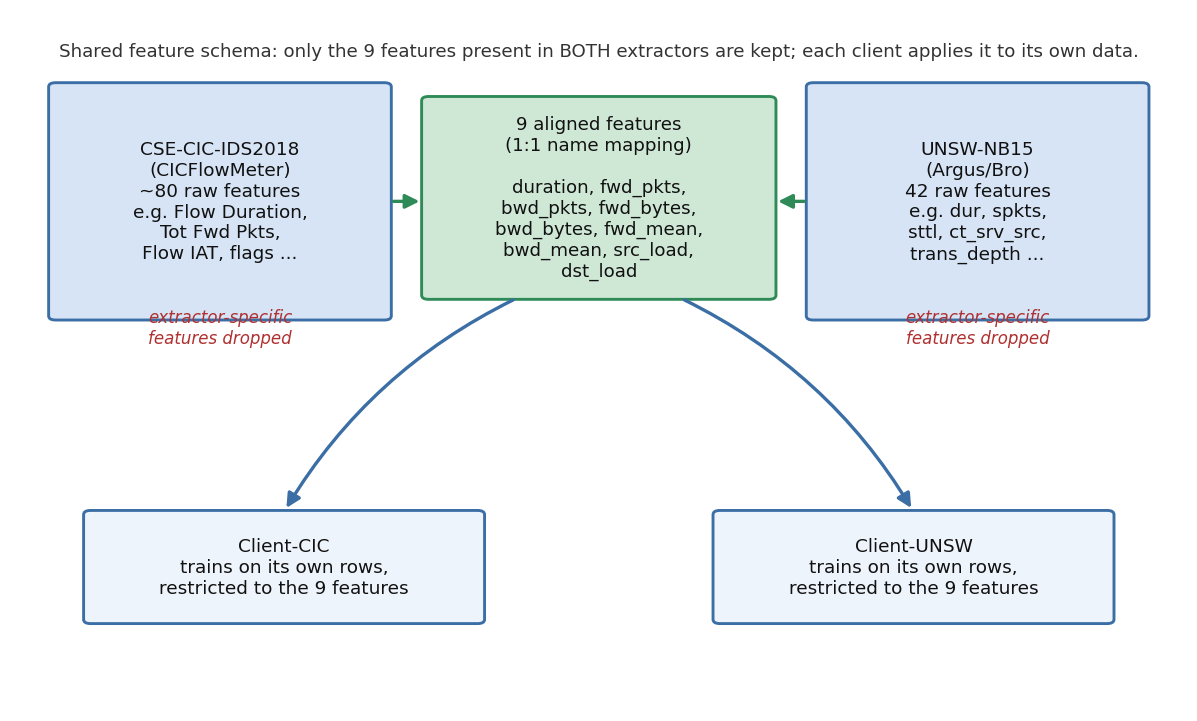
\includegraphics[width=\columnwidth]{fig_feature_alignment.png}}
\caption{Cross-dataset feature alignment.}
\label{fig:align}
\end{figure}

\subsection{Federated Architecture}
Our federation follows a horizontal cross-silo pattern with one aggregator and two
clients, each holding one dataset: Client-CIC and Client-UNSW (Fig.~\ref{fig:arch}).
Each client trains on its own data without ever sending raw data; only model weights
are exchanged. Feature normalization (z-score) is also computed locally per client, so
no data statistics leak between clients. Each round, the aggregator sends the global
model; each client trains locally and returns a weight update; the aggregator combines
the updates with FedAvg (weighted by data size) to form the next global model, for 100
rounds. In practice the three nodes run as three \texttt{t3.medium} EC2 instances with
weights exchanged via Amazon S3, but this is operational detail that does not change
the FL model itself.

\begin{figure}[htbp]
\centerline{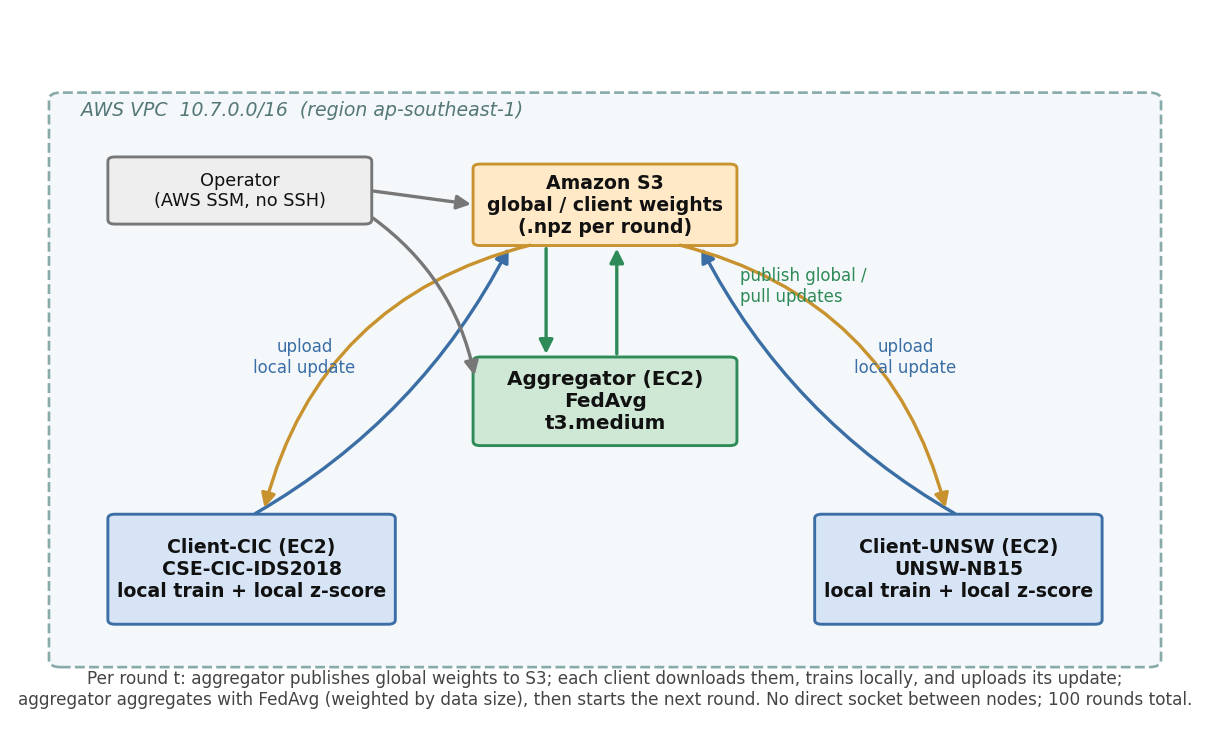
\includegraphics[width=0.85\columnwidth]{fig_fl_architecture.png}}
\caption{Federated learning architecture.}
\label{fig:arch}
\end{figure}

\subsection{Claims and Metrics}
We test six representative claims, grouped as reproduction (R1--R4) and adversarial
(R5--R6): R1 FedAvg versus FedProx; R2 non-IID impact (Dirichlet $\alpha$ sweep); R3
cross-dataset FL feasibility; R4 real cloud cost; R5 evasion vulnerability (FGSM, PGD,
JSMA with constrained perturbations); and R6 adversarial training as a defense. The
primary metric is the Matthews correlation coefficient (MCC), which stays reliable
under heavy class imbalance; we also report recall, precision, and attack success rate
(ASR). Experiments use the seeds $\{13,42,101,202,303\}$.

\section{Results and Discussion}
\label{sec:results}
Table~\ref{tab:results} summarizes the verification. We report every result as-is,
including where a claim does not hold.

\textit{R1 (FedProx vs.\ FedAvg): does not hold.} On the cross-dataset setting, FedAvg
and FedProx are statistically indistinguishable (MCC 0.572 vs.\ 0.571; difference about
0.001), and both converge in 7--11 rounds. FedProx does not improve on FedAvg over the
hyperparameter range we tested.

\textit{R2 (non-IID impact): domain dependent.} On Client-CIC the classic pattern
appears---MCC falls from 0.512 at $\alpha{=}100$ to 0.387 at $\alpha{=}0.1$ and becomes
highly unstable---whereas on Client-UNSW performance stays flat or even rises (0.621 to
0.655), because UNSW classes are relatively easy to separate. The claim ``non-IID
harms FL'' therefore holds for CIC but not for UNSW: the effect is real but not
universal.

\textit{R3 (cross-dataset FL is hard): holds strongly.} The federated model collapses
to MCC $-0.026$ (recall 0.058), essentially random, while a centralized upper bound
(data pooled, not allowed in real FL) reaches only 0.545 and local-only models are also
poor. Merging two very different networks via FedAvg and nine generic aligned features
fails to transfer.

\textit{R4 (cloud cost): measured.} With a light 9{,}601-parameter model, each client
upload is 76.8~KB, so aggregator traffic is about 300~KB per round for two clients.
From S3 object timestamps, 100 rounds take about 27 minutes (about 16 seconds per round
including S3 sync), measured while two runs shared CPU.

\textit{R5 (evasion vulnerability): holds strongly.} Even at a small budget
($\epsilon{=}0.05$) the attack success rate is already 0.96 for all three attacks; at
$\epsilon{\geq}0.2$, FGSM and PGD reach ASR 1.00, pushing MCC from $-0.026$ to $-0.15$.
The cross-dataset FL model is almost fully evadable.

\textit{R6 (adversarial training as defense): does not hold here.} Adversarial training
slightly raises clean MCC ($-0.026 \rightarrow 0.070$) but fails on robustness: MCC
under PGD worsens ($-0.152 \rightarrow -0.222$). Adding adversarial examples to an
already weak cross-dataset FL model does not restore evasion robustness. (Absolute MCC
is low in R5--R6 because the R3 baseline itself collapses; values are read as direction,
not absolute performance.)

As a sanity check that federation helps, the federated model beats a local-only
baseline across five seeds (MCC 0.574 vs.\ 0.364; paired $t$-test $p{=}0.0005$).

Two caveats frame these results. First, verification measures whether the
\emph{direction} of a claim holds on a uniform testbed, not an exact replication of the
original setup, so absolute differences from the original papers are expected. Second,
our adversarial experiments act on the tabular flow-feature space, not raw packets:
FGSM/PGD/JSMA perturbations are constrained so flows stay valid, making the attacks
more conservative than unconstrained image-domain attacks.

\begin{table}[htbp]
\caption{Verification results for the six FL-NIDS claims.}
\label{tab:results}
\begin{center}
\footnotesize
\begin{tabular}{|l|l|c|}
\hline
\textbf{Claim} & \textbf{Our lab result} & \textbf{Holds?} \\
\hline
R1 FedProx$>$FedAvg & 0.572 vs.\ 0.571, n.s. & No \\
R2 non-IID harms FL & CIC drops; UNSW flat & Domain dep. \\
R3 cross-dataset hard & fed.\ $-0.03$ vs.\ cen.\ 0.55 & Yes \\
R4 comm.\ cost & 300 KB, 16 s / round & --- \\
R5 evasion & ASR 0.96--1.00 & Yes \\
R6 adv.\ training & clean up, robust worse & No \\
\hline
\end{tabular}
\end{center}
\end{table}

From these findings, the most pressing research directions are semantic-aware feature
alignment to improve cross-dataset transfer, direction- and domain-aware evasion
defenses instead of static adversarial training, leakage-free cross-dataset evaluation
protocols, and validation at a client and traffic scale closer to production.

\section{Conclusion}
This survey combines a thematic review of recent FL-NIDS literature with something
rarely done: reproducible verification of its representative claims on a uniform AWS
testbed. Rather than summarizing what original authors reported, we re-test whether each
claim holds in an equivalent environment and report the outcome honestly. Of six
claims, two hold (cross-dataset FL is hard; models are highly evadable), one is domain
dependent (non-IID impact), and two do not hold (FedProx over FedAvg; adversarial
training restoring robustness). The main contribution is evidence: a reproducible,
reasonably priced baseline that shows clearly which FL-NIDS claims are robust and which
are fragile under controlled testing. All protocols, scripts, and cloud configurations
are made available so the community can reproduce and build upon them.

\section*{Acknowledgment}
The authors thank Politeknik Elektronika Negeri Surabaya (PENS) for computing support.

\begin{thebibliography}{00}
\bibitem{b1} A. Khraisat, A. Alazab, T. Jan, and A. Gopez, ``Survey on federated learning for intrusion detection system: concept, architectures, aggregation strategies, challenges, and future directions,'' ACM Comput. Surv., 2024.
\bibitem{b2} J. L. Hernandez-Ramos et al., ``Intrusion detection based on federated learning: a systematic review,'' ACM Comput. Surv., 2025.
\bibitem{b3} A. A. Wardana and P. Sukarno, ``Taxonomy and survey of collaborative intrusion detection system using federated learning,'' ACM Comput. Surv., 2024.
\bibitem{b4} E. V. Fedorchenko, E. Novikova, and A. N. Shulepov, ``Comparative review of the intrusion detection systems based on federated learning: advantages and open challenges,'' Algorithms, vol. 15, no. 7, p. 247, 2022.
\bibitem{b5} L. Lavaur, Y. Busnel, and F. Autrel, ``Demo: highlighting the limits of federated learning in intrusion detection,'' in Proc. IEEE ICDCS, 2024, pp. 1416--1419.
\bibitem{b6} J. Zhang et al., ``Combating exacerbated heterogeneity for robust models in federated learning (SFAT),'' arXiv:2303.00250, 2023.
\bibitem{b7} S. Saha, M. I. Sayed, M. Faezipour, and S. Bhatt, ``Resilient federated learning for DDoS detection with multi-Krum aggregation and anomaly detection,'' in Proc. IEEE SmartNets, 2025.
\bibitem{b8} S. Saini, A. Chennamaneni, and B. A. Sawyerr, ``A review of the duality of adversarial learning in network intrusion: attacks and countermeasures,'' arXiv:2412.13880, 2024.
\bibitem{b9} Y. Hu, J. Wu, G. Li, J. Li, and J. Cheng, ``Privacy-preserving few-shot traffic detection against advanced persistent threats via federated meta learning,'' IEEE Trans. Netw. Sci. Eng., vol. 11, pp. 2549--2560, 2024.
\bibitem{b10} O. Ceviz, S. Sen, and P. Sadioglu, ``Distributed intrusion detection in dynamic networks of UAVs using few-shot federated learning,'' arXiv:2501.13213, 2025.
\bibitem{b11} J. Xu, C. Li, Y. Zheng, and Z. Li, ``Entente: cross-silo intrusion detection on network log graphs with federated learning,'' arXiv:2503.14284, 2025.
\bibitem{b12} Z. Chen, N. Lv, P. Li, Y. Fang, K. Chen, and W. Pan, ``Intrusion detection for wireless edge networks based on federated learning,'' IEEE Access, vol. 8, pp. 217463--217472, 2020.
\bibitem{b13} J. Mao, Z. Wei, B. Li, R. Zhang, and L. Song, ``FedIn-NID: a federated learning framework for network intrusion detection in large-scale heterogeneous industrial IoT,'' IEEE Trans. Inf. Forensics Security, 2025.
\bibitem{b14} R. Doriguzzi-Corin and D. Siracusa, ``FLAD: adaptive federated learning for DDoS attack detection,'' arXiv:2205.06661, 2022.
\bibitem{b15} R. Doriguzzi-Corin, S. Cretti, and D. Siracusa, ``Resource-efficient federated learning for network intrusion detection,'' in Proc. IEEE NetSoft, 2024.
\bibitem{b16} G. Singh, K. Singh, P. Rajalakshmi, and Y. Xong, ``Sentinel: dynamic knowledge distillation for personalized federated intrusion detection in heterogeneous IoT networks,'' arXiv:2510.23019, 2025.
\bibitem{b17} Y.-C. Lee, W.-C. Chien, and Y.-C. Chang, ``FedDB: a federated learning approach using DBSCAN for DDoS attack detection,'' Appl. Sci., vol. 14, no. 22, 2024.
\bibitem{b18} M. Khalid, U. Zukaib, M. Al-Rakhami, and A. M. Alamri, ``FedCross-VAN: federated cross-domain behavior alignment for VANET intrusion detection,'' Trans. Emerg. Telecommun. Technol., vol. 37, 2025.
\bibitem{b19} S. Ali, R. Alireza, and A. Mahmood, ``Mist-assisted federated learning for intrusion detection in heterogeneous IoT networks,'' arXiv:2511.00271, 2025.
\bibitem{b20} M. Benkaddour, ``Enhancing federated learning for privacy preserving intrusion detection in IoT networks,'' Przeglad Elektrotechniczny, 2025.
\bibitem{b21} E. M. Ennaji, S. E. Hajla, Y. Maleh, and S. Mounir, ``Adversarially robust federated deep learning models for intrusion detection in IoT,'' Indones. J. Electr. Eng. Comput. Sci., vol. 37, no. 2, p. 937, 2024.
\bibitem{b22} G. Chandu, T. S. Karthik, and B. Parag, ``Federated learning for distributed IoT security: a privacy-preserving approach to intrusion detection,'' IEEE Access, 2025.
\bibitem{b23} S. K. Ghimire and S. Lodh, ``FedSecIoT: a federated learning framework for collaborative and privacy-preserving botnet detection in IoT with adversarial robustness,'' in Proc. IEEE SILCON, 2025.
\bibitem{b24} A. Al Mazroa et al., ``FORT-IDS: a federated, optimized, robust and trustworthy intrusion detection system for IIoT security,'' Sci. Rep., 2025.
\bibitem{b25} M. S. I. Sajid et al., ``GADoT: GAN-based adversarial training for robust DDoS attack detection,'' arXiv:2201.13102, 2022.
\bibitem{b26} H. Dadhwal, M. de Abreu, N. Parvizi, and S. Saha, ``Benchmarking the adversarial resilience of machine learning models for DDoS detection,'' Array, vol. 29, p. 100664, 2026.
\bibitem{b27} I. Debicha, T. Debatty, J.-M. Dricot, and W. Mees, ``Adversarial training for deep learning-based intrusion detection systems,'' arXiv:2104.09852, 2021.
\bibitem{b28} Q. Mao, X. Lin, G. Li, and J. Li, ``FeCoGraph: label-aware federated graph contrastive learning for few-shot network intrusion detection,'' IEEE Trans. Inf. Forensics Security, 2025.
\bibitem{b29} K. Yin, J. Zhang, Z. Xia, and C. Yu, ``FedPKT: robust cross-domain few-shot intrusion detection via prototypical knowledge transfer,'' IEEE Trans. (early access), 2025.
\bibitem{b30} K. S, V. Malathi, B. J. Lakshmi, A. V. Sriharsha, T. D. Kumar, and T. Lakshmibai, ``Federated and explainable intrusion detection systems for large-scale heterogeneous networks using ensemble deep learning,'' in Proc. IEEE ICACRS, 2025.
\end{thebibliography}

\end{document}
